% !TEX TS-program = pdflatex
% !TEX encoding = UTF-8 Unicode

% This is a simple template for a LaTeX document using the "article" class.
% See "book", "report", "letter" for other types of document.

\documentclass[11pt]{article} % use larger type; default would be 10pt

\usepackage[utf8]{inputenc} % set input encoding (not needed with XeLaTeX)

%%% Examples of Article customizations
% These packages are optional, depending whether you want the features they provide.
% See the LaTeX Companion or other references for full information.

%%% PAGE DIMENSIONS
\usepackage{geometry} % to change the page dimensions
\geometry{a4paper} % or letterpaper (US) or a5paper or....
% \geometry{margin=2in} % for example, change the margins to 2 inches all round
% \geometry{landscape} % set up the page for landscape
%   read geometry.pdf for detailed page layout information

\usepackage{graphicx} % support the \includegraphics command and options

% \usepackage[parfill]{parskip} % Activate to begin paragraphs with an empty line rather than an indent

%%% PACKAGES
%\usepackage{booktabs} % for much better looking tables
%\usepackage{array} % for better arrays (eg matrices) in maths
%\usepackage{verbatim} % adds environment for commenting out blocks of text & for better verbatim
%\usepackage{subfig} % make it possible to include more than one captioned figure/table in a single float
% These packages are all incorporated in the memoir class to one degree or another...


%%% HEADERS & FOOTERS
\usepackage{fancyhdr} % This should be set AFTER setting up the page geometry
\pagestyle{fancy} % options: empty , plain , fancy
\renewcommand{\headrulewidth}{0pt} % customise the layout...
\lhead{}\chead{}\rhead{\textcopyright \ Andrea Donati}
\lfoot{A.A. 2017/2018}\cfoot{\thepage}\rfoot{Prof. Stefano Ceri}

%%% SECTION TITLE APPEARANCE
%\usepackage{sectsty}
%\allsectionsfont{\sffamily\mdseries\upshape} % (See the fntguide.pdf for font help)
% (This matches ConTeXt defaults)

%%% ToC (table of contents) APPEARANCE
%\usepackage[nottoc,notlof,notlot]{tocbibind} % Put the bibliography in the ToC
%\usepackage[titles,subfigure]{tocloft} % Alter the style of the Table of Contents
%\renewcommand{\cftsecfont}{\rmfamily\mdseries\upshape}
%\renewcommand{\cftsecpagefont}{\rmfamily\mdseries\upshape} % No bold!

%%% END Article customizations

%%% The "real" document content comes below...

\title{Appunti di Basi di Dati 1}
\author{Andrea Donati}
\date{A.A. 2017/2018 - Prof. Stefano Ceri} % Activate to display a given date or no date (if empty),
         % otherwise the current date is printed 

\begin{document}
\maketitle

\newpage
\tableofcontents
\newpage

\section{Introduzione}

I dati sono il cuore dei sistemi informatici, nessuna impresa può operare senza aver sviluppato e formalizzato la modalità di accesso e gestione dei propri dati. In quanto "patrimonio aziendale", essi devono essere gestiti e protetti.\\
Un \bf dato \rm a se stante è poco utile, è l'unità elementare grezza dell'informazione. Quest'ultima può essere definita come l'\bf elaborazione \rm dei dati per rispondere a esigenze specifiche dell'impresa. \\
\\
Un esempio di \bf dato \rm può essere: "Stefano Ceri, Basi di dati, IIIA, I Sem". Da questo dato possiamo estrarre le seguenti informazioni:\\
\begin{itemize}
\item Chi insegna questa materia? Stefano Ceri
\item Quando si tiene il corso? Al I semestre del III anno.
\end{itemize}

\noindent Questa distinzione swag.

\section{Modelli dei Dati}

I modelli costituiscono una strutturazione semplificata della realtà, che ne coglie gli aspetti specifici ed aiuta a comprenderla meglio.\ Esempi dei \bf modelli logici \rm più comuni sono: il modello Gerarchico, il modello Reticolare e il modello Relazionale, sul quale concentreremo la nostra attenzione.

\subsubsection{Il Modello Gerarchico e il Modello Reticolare}
Queste due strutture sono molto simili, nel senso che in entrambe i dati sono rappresentati in raggruppamenti come \bf record \rm, mentre le associazioni tra i dati sono differenti per i due modelli.\\
Nel modello \bf Gerarchico \rm sono rappresentate con \bf puntatori \rm in una struttura ad albero, mentre nel modello \bf Reticolare \rm come \bf puntatori \rm in una struttura a grafo complesso.
\subsubsection{Il Modello Relazionale} nel modello relazionale i dati sono invece rappresentati come \bf tabelle \rm, mentre le associazioni tra i dati sono ottenute associando i \bf valori \rm di attributi in tabelle diverse.\\
Una definizione formale del modello Relazionale può essere la seguente:
\begin{description}
\item[Dominio] qualunque insieme di valori;
\item[Prodotto Cartesiano su n domini \(D\textsubscript 1 \times ... \times D\textsubscript n\) non necessariamente distinti] insieme delle tuple \( "d\textsubscript 1, ... , d\textsubscript n" \) con \( d\textsubscript i  \in D\textsubscript i \) ed \(1 \le i \le n;\)
\item[Relazione su \(D\textsubscript 1 \times ... \times D\textsubscript n\)] un qualunque sottoinsieme di D\textsubscript 1 x ... x D\textsubscript n.
\end{description}
\noindent Le \bf Relazioni \rm hanno diverse proprietà utili:
\begin{description}
\item[Grado della Relazione] numero di domini coinvolti;
\item[Cardinalità della Relazione] numero di tuple che la compongono;
\item[Attributo] nome dato ad un dominio in una relazione. I nomi di attributi devono essere tutti distinti tra loro. 
\end{description}
\noindent Lo \bf schema di una Relazione \rm è il modo in cui la si rappresenta formalmente. \\ Si scrive come \( R(attributo1, ... , attributoN)\) ed è importante ricordare che anche i nomi delle relazioni in uno stesso schema devono essere univoci.\\
Queste definizioni ad un primo impatto possono risultare fuorvianti per uno studente alle prime armi, si può però fare un esempio di corrispondenza tra definizioni formali e definzioni informali (usate nel linguaggio comune).\\
Una \bf Relazione \rm è comunemente vista come una Tabella, mentre un \bf attributo \rm come la Colonna di una Tabella.\ 
Una \bf Tupla \rm è una riga della Tabella, il \bf Dominio \rm è il tipo del dato e la \bf Cardinalità \rm è il numero di righe, mentre il \bf grado \rm è il numero di colonne.

\paragraph{Interrogazioni} Le interrogazioni (eseguite tramite un \it Query Language\rm) sono ciò che permette di passare dal dato all'informazione. Una volta ottenuto uno schema di organizzazione dei dati, come esemplificato nell'introduzione, è possibile ricavarne informazione tramite interrogazioni. Le interrogazioni dovranno ovviamente essere coerenti con i dati raccolti.\\
Al fine di eseguire in modo ottimale le interrogazioni su un \it database \rm conviene arricchire lo schema, aggiungendo dei \bf Vincoli di Integrità\rm.
\paragraph{Vincoli di Integrità} Escludono alcune possibili istanze della relazione in quanto non rappresentano concretamente il mondo applicativo. Infatti, è possibile che determinate combinazioni di dati dei diversi domini che compongono la relazione non abbiano "senso" nella realtà che stiamo considerando.\\
Tali vincoli possono essere, ad esempio:
\begin{itemize}
\item \bf Chiavi \rm
\item \bf Vincoli su valori nulli \rm
\item \bf Integrità Referenziale \rm
\item \bf Vincoli Generici \rm
\end{itemize}
\noindent In particolare, la \bf Chiave \rm ha un ruolo importante nel database, è definita come sottoinsieme di attributi dello schema con le proprietà di \it Unicità\rm, ossia non possono esistere due tuple con l'attributo chiave uguale, e \it Minimalità\rm, ossia, sottraendo un qualunque attributo alla chiave si perde la proprietà di unicità.\\
Di seguito un esempio, più o meno, riassuntivo.
\begin{figure}[htbp]
		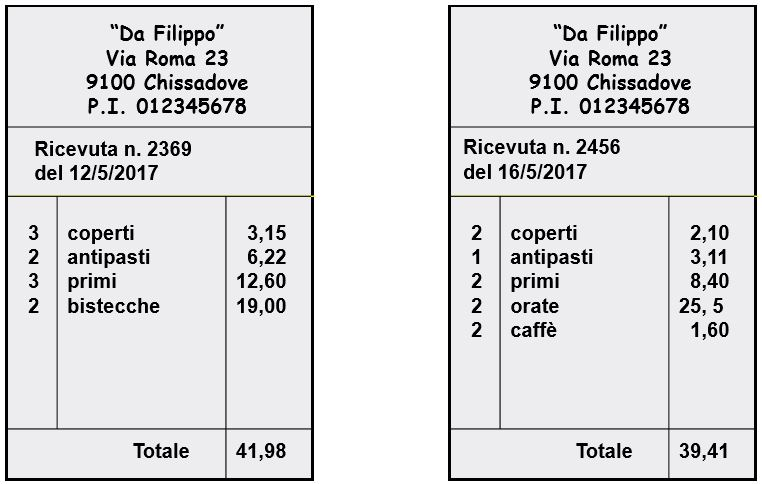
\includegraphics{IstanzeRicevutaFiscale.jpg}
	\caption{Esempio di due istanze di ricevuta fiscale.}
\end{figure}
\begin{figure}[htbp]
		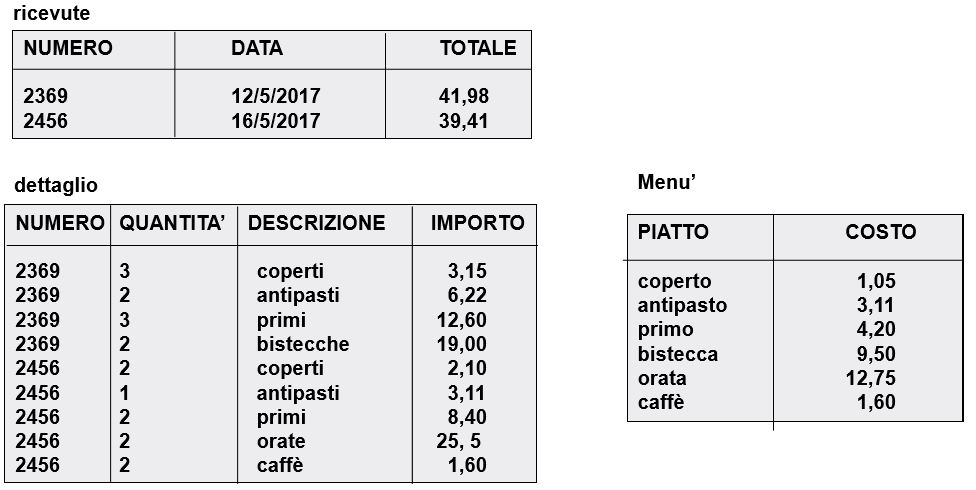
\includegraphics{ModelloRelazionaleRicevuteFiscali.jpg}
	\caption{Esempio del \bf modello relazionale \rm derivante dalle ricevute fiscali.}
\end{figure}
\newpage
\section{Algebra Relazionale}
L'Algebra Relazionale, definita da Codd nel 1970, è un utile strumento per imparare a formulare query corrette. Si compone di un insieme minimo di 5 operazioni, la cui combinazione dà l'intero potere espressivo del linguaggio. Le operazioni dell'Algebra Relazionale sono indicate di seguito. (Inserire immagine "Una visione d'insieme" delle operazioni.)
\subsection{Selezione}
Supponiamo di avere di avere una Relazione STUDENTE composta dei domini Matricola, Nome, Città, ecc..\\
Indicata come $$ \sigma \textsubscript{ Nome = "Paola"}\  STUDENTE $$, la selezione produce una Tabella, \bf priva di nome \rm che ha per Schema lo stesso Schema di STUDENTE, e per Istanza le Tuple di STUDENTE che soddisfano il predicato di selezione.\\
La sintassi del predicato di Selezione permette di utilizzare espressioni booleane di predicati semplici al suo interno.
\subsection{Proiezione}
Indicata con $$ \sqcap \textsubscript{ Nome, Città}\  STUDENTE $$ la Proiezione produce una tabella, \bf priva di nome \rm con Schema gli attributi Nome e Città, ossia quelli indicati al pedice del predicato, e come Istanze la restrizione delle Tuple di STUDENTE (argomento del predicato) agli attributi (a.k.a. campi, domini) Nome e Città.\\
Va specificato che nel modello \bf formale \rm, la Proiezione elimina eventiuali duplicati prodotti implicitamente, ma nel modello \bf informale \rm (e nel modello effettivamente implementato nei Sistemi) l'eliminazione di duplicati va richiesta esplicitamente.
\subsection{Assegnamento}
Non è una vera e propria operazione algebrica dell'Algebra Relazionale, ma è comunque utile e molto usata dato che permette di dare un nome al risultato di un'espressione algebrica. Ad esempio $$ INFORMATICI = \sigma \textsubscript{CorsoStudi = "Informatica"}\  STUDENTE.$$ In pratica al risultato prodotto dalle operazioni algebriche, che abbiamo detto essere senza nome, possiamo in questo modo assegnare un nome.
\subsection{Unione}
$$ Tabella1\  \cup\  Tabella2 $$ è possibile eseguire l'unione di due tabelle solo se esse sono \bf compatibili\rm, ossia con lo stesso grado. Nella realtà applicativa è possibile unire due tabelle solamente se esse hanno domini \it ordinatamente dello stesso tipo.\rm\\
L'operazione algebrica di Unione produce un risultato che è una Tabella (priva di nome) che ha per Schema lo stesso Schema di Tabella1, e per Istanze l'unione delle tuple di Tabella1 e Tabella2.
\subsection{Differenza}
Indicata con $$ Tabella1\ -\ Tabella2 $$, si può fare solamente se le due tabelle argomento sono \bf compatibili\rm. Produce una tabella priva di nome che ha per Schema lo stesso Schema di Tabella1 e come Istanze la differenza delle tuple di Tabella1 e Tabella2.
\subsection{Prodotto Cartesiano}
Indicata con $$ R\ \times\ S $$ produce una tabella, piva di nome, con Schema l'unione degli attributi di R ed S (quindi il grado di \( (R \times S) = grado(R) + grado(S)\)), e come Istanze tutte le possibili coppie di tuple di R ed S (quindi la cardinalità di \( (R \times S) = card(R) * card(S)\)).
\subsection{Intersezione}
Indicata con $$ R\ \cap\ S $$, l'operazione algebrica di intersezione ha senso solamente quando R ed S sono compatibili (come per gli altri operatori algebrici/insiemistici visti in precedenza).\\
L'intersezione è derivabile tramite la seguente formula: \( R \cap S = R - (R - S) \) e produce come risultato una tabella con lo stesso Schema di R e come Istanze l'intersezione delle tuple di R ed S.
\subsection{Join}
Indicata con $$ STUDENTE\  \bowtie \textsubscript{STUDENTE.Matr = ESAME.Matr}\  ESAME $$ ha come espressione equivalente (operatore derivato) la seguente $$ \sigma \textsubscript{STUDENTE.Matr = ESAME.Matr} \ STUDENTE\ \times\ ESAME. $$
La notazione puntata è usata per rendere non ambigua l'espressione, quindi per differenziare attributi omonimi all'interno di tabelle diverse. Produce una tabelle, priva di nome, con Schema la \bf concatenazione \rm degli Schemi della prima e della seconda tabella e come Istanze le tuple ottenute concatenando quelle tuple di STUDENTE e di ESAME che soddisfano il predicato.\\
Il Join si differenzia in vari sottotipi.
\subsubsection{Join Naturale} equi-join di tutti gli attributi omonimi (si omette il predicato, si elimina la colonna ripetuta).
\subsubsection{Semi Join} produce una tabella con Schema lo stesso schema di STUDENTE e come Istanze la proiezione su STUDENTE del Join tra STUDENTE ed ESAME. In parole povere restituisce una tabella (priva di nome) contenente le sole tuple di STUDENTE che rispettano la condizione di Join con ESAME.\\
Un'espressione equivalente è $$ \sqcap \textsubscript{Attr(STUDENTE)} STUDENTE \bowtie \textsubscript{STUDENTE.Matr = ESAME.Matr} ESAME. $$
\subsubsection{Semi-Join Naturale} proietta su STUDENTE (Semi Join) il Join Naturale di studente ed ESAME.
\subsection{Ottimizzazione delle Interrogazoni}
Eisitono molte diverse soluzioni per uno stesso problema di interrogazione, e le soluzioni che producono lo stesso risultato sono considerate fra loro \bf equivalenti\rm. Alcune di queste espressioni. però riescono a essere più efficienti di altre.\\
Considerando questo, è naturale volere ottenere sempre delle interrogazioni che svolgono il loro compito più velocemente delle loro alternative. Per ottenere la forma algebrica ottimizzata di una interrogazione dobbiamo stabilire i criteri di ottimizzazione, e per questo scopo conviene utilizzare una rappresentazione della struttura dell'interrogazione \bf ad albero\rm. \\ \\
Ogni espressione dell'algebra relazionale può essere rappresentata in modo grafico da un albero, che esplicita l'ordine di valutazione degli operatori. In questa struttura, ogni operatore corrisponde ad un nodo dell'albero, i cui argomenti sono i nodi figli. Gli operatori unari avranno un ramo in ingreso e un ramo in uscita, mentre quelli binari avranno due rami in ingresso ed uno in uscita.\\
Abbiamo quindi una serie di \bf trasformazioni di equivalenza\rm, la quale lettura è consigliata sulle slide messe a disposizione dal docente.
\newpage
\section{Calcolo Relazionale}
Il calcolo relazionale si compone di una famiglia di linguaggi formali, come il Calcolo delle Tuple \bf TRC \rm e il Calcolo dei Domini \bf DRC\rm. TRC in particolare è diviso in due versioni, con tuple ristrette sul range e con tuple arbitrarie, il nostro caso di studio si concentrerà sul TRC a tuple arbitrarie.
\subsubsection{TRC a Tuple Arbitrarie}
TRC, come la maggio parte dei linguaggi relazionali, è un linguaggio di tipo dichiarativo, nel senso che si limta ad esprimere la descrizione del risultato del calcolo, ma non il metodo operativo tramite cui ottenerlo.
\paragraph{Definizione Formale di TRC}
\begin{itemize}
\item Forma Standard: \( \{ t\  |\  p(t) \} \), dove \( p(t) \) è una \bf formula \rm costruita tramite \bf atomi\rm.
\item Un \bf atomo\rm\ può essere uno scalare o un'espressione del tipo\\ \it espressione - comparatore - espressione. \rm Un'espressione usa costanti e restrizioni sull'attributo A di una tupla t, tali restrizioni si indicano con t[A].\\
Cosa importante è che un atomo deve essere una \bf formula ben formata \rm (vedi logica del prim'ordine).
\end{itemize}
\paragraph{Correttezza delle Formule}
Si considerano corrette solamente le formule la cui soluzione è indipendente dal dominio, ma dipende solamente dalle istanze del database.\\
Si definiscono formule \bf unsafe \rm le formule che danno un risultato infinito, come ad esempio \( \{ t | t \notin \Re \} \).
\newpage
\section{Datalog}
Datalog è un linguaggio di \it programmazione logica \rm basato su "formule", che prendono il nome di \bf regole\rm. Ogni regola è composta da una Testa (Head o LHS) ed un Corpo (Body o RHS) e si scrive come $$ P\ :-\ P\textsubscript{1}, ... , P\textsubscript{n} $$ dove ogni P rappresenta un \bf predicato \rm (o letterale) composto da un nome e degli argomenti, che possono essere variabili, costanti o "don't care" (qualsiasi elemento). Un esempio di regola può essere $$ persona(\ X\ ,\ \_\_\  ,\ M\ ). $$ L'\bf interpretazione \rm di una regola Datalog è vera se il corpo della regola è vero, ed è importante specificare che le variabili non esplicitamente quantificate all'interno della regola si intendono come quantificate \it esistenzialmente\rm.\\ Per esemplificare i concetti e le regole del Datalog useremo la seguente Base di Dati.
\begin{figure}[htbp]
		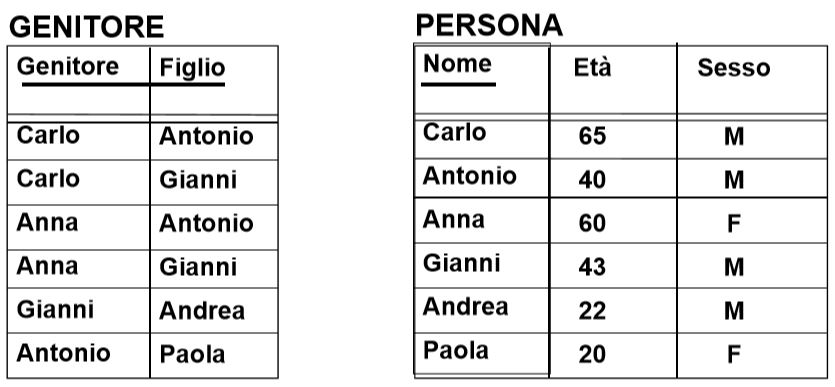
\includegraphics{BaseDatiEsempioDatalog.jpg}
	\caption{Base di Dati di esempio per le regole Datalog.}
\end{figure}
\newpage
\subsection{Fatti e Goal}
Per \bf Fatto \rm in Datalog si intende il letterale \it ground\rm, per esempio $$ Genitore("Carlo","Antonio") $$ ed è in diretta corrispondenza con la \bf Tupla \rm di un database. \\
Un \bf Goal \rm corrisponde invece ad una Query. $$ ?-\ Padre("Carlo", X) $$ ed è valutata cercando una regola che abbia per Testa il predicato, nell'esempio, "Padre" e unificando tutte le cariabili X che rendono la regola vera. Il risultato del Goal di esempio è $$ X = \{ "Antonio", "Gianni" \}.$$ Esistono Goal nei quali non sono epresse variabili, questi restituiscono \it True o Fase \rm. Esempi: $$ ? - Padre("Carlo","Antonio") \Rightarrow True $$ $$ ? - Padre("Carlo","Andrea") \Rightarrow False. $$ \\
\subsection{Esempi di Regole}
Di seguito alcuni esempi di regole Datalog con spiegazione:
$$ Nonno(X,Z) :- Padre(X,Y), Genitore(Y,Z) $$
Questa Regola, sinteticamente, esprime in che modo un elemento X può essere considerato "Nonno" di un elemento Z. Infatti la Testa della regola è composta dal predicato $"Nonno"$ che è vero, in base a quanto detto sulle regole, solamente quando il corpo è vero.\\
Il corpo della regola è composto dai predicati $"Padre"$ e $"Genitore"$, separati da una virola che va interpretata come un \it Prodotto Logico (AND).\rm Questa specifica regola si presta ad una lettura intuitiva, perchè un elemento X sia "Nonno" di un elemento Z è necessario che esista un elemento Y (dato che Y è quantificata esistenzialmente in modo implicito), del quale X è padre, tale che Y è genitore di Z.\\
$$Fratello(X,Y) :- Genitore(Z,X), Genitore(Z,Y), X \not = Y$$
Anche questa regola, come quella precedente, ha una lettura intuitiva. Esprime in che modo un elemento X è considerato "Fratello" di un elemento Y, cioè quando esiste un elemento Z (quantificato esistenzialmente nella regol in modo implicito), che è genitore di X e di Y, quando X e Y sono due elementi diversi (escudiamo quindi la possibilità che un elemento sia "Fratello" di sè stesso).\\
$$Zio(X,Y) :- Persona(X,\_\_,"M"), Fratello(X,Z), Genitore(Z,Y)$$
In questa regola vediamo il primo esempio di "don't care", un simbolo speciale utilizzato per indicare un parametro di cui non ci interessa il valore. In questo caso il "don't care" è l'età della persona che possiamo considerare "Zio". Dovrebbe essere immediata a questo punto la lettura della suddetta regola. Consideriamo un elemento X "Zio" di un elemento Y quando: X è una persona di sesso maschile della quale non ci interessa l'età ed esiste un elemento Z, di cui X è fratello, tale che Z è genitore di Y.
\subsection{Negazione}
Ovviamente per scrivere regole Datalog è possibile usare la negazione (anzi, essa aumenta il potere espressivo del linguaggio), essa però introduce dei problemi in quanto a correttezza. Ad esempio $$ q(x) :- \sim p(X) $$ $$p(0) $$ \bf Non \rm è safe! Perchè $$ ?- p(0) $$ produce un risultato \bf infinito\rm. \\
Per usare correttamente l'operatore di negazione è necessario che la regola abbia 2 proprietà:
\begin{itemize}
\item La negazione deve essere \bf safe\rm. Tutte le variabili di un letterale negato devono comparire anche in un letterale positivo all'interno della regola. $$ P(X) :-\ R(X), \sim P(X)  $$ Non è corretta.
\item La negazione deve essere \bf stratificata\rm. Ossia non ci devono essere cicli di dipendenza tra letterali negati.
\end{itemize}
A fronte di questi accorgimenti, la negazione aumenta il potere espressivo di Datalog, superando anche quello dell'Algrbra Relazionale, per il fatto di poter scrivere Query \bf ricorsive\rm.
\subsection{Query Ricorsive}
Una Query ricorsiva si distingue dalle altre perchè contiene all'interno del corpo della regola anche il letterale di testa. Ad esempio: $$ Start: Antenato(X,Y) :- Genitore(X,Y) $$
$$ Ricorsione: Antenato(X,Y) :- Antenato(X,Z), Genitore(Z,Y) $$
Il meccanismo di valutazione di una Query Datalog ricorsiva è molto simile a quello usato per il risolutore di un insieme di clausule (vedi corso di Logica e Algebra), valutando ad ogni passo la Query corrente e unendo il risultato alla Query del passo ricorsivo precedente, fino a quando $$ Antenato \textsuperscript{n} = Antenato \textsuperscript{n-1}  $$cioè si raggiunge il \bf punto fisso\rm.\\
La negazione descritta sopra può causare grandi problemi con questo tipo di Query. Ad esempio, la seguente Query
$$ Antenato(X,Y) :- Genitore(X,Y) $$
$$ Antenato(X,Y) :- Antenato(X,Z),Genitore(Z,Y) $$
$$ Non-ant (X,Y) :- Persona(X,\_,\_), Persona (Y,\_,\_), \sim Antenato(X,Y) $$
se valutata nel modo che abbiamo descritto prima produce un risultato sbagliato, poichè al primo passo di iterazione, calcoliamo NON-ANT sottraendo il valore corrente della relazione ANTENATO (che è uguale a GENITORE) dal prodotto cartesiano delle persone. Al secondo passo di iterazione, aggiungiamo al valore precedente di  NONANT il nuovo valore computato, che sarà \bf più piccolo\rm, etc. quindi NON-ANT non varia più. \\
Il risultato finale sarà scorretto, perché conterrà tutte  le persone che non hanno tra loro un rapporto genitore-figlio. \\
Questo succede perchè non si è rispettata la proprietà di \it stratificazione \rm della Query ricorsiva, la proprietà della negazione che abbiamo descritta come necessaria in precedenza.\\
Lo stesso programma Datalog riscritto stratificato produce un risultato corretto ed è anche di più facile lettura:\\
Strato 1: 
$$Antenato(X,Y) :- Genitore(X,Y)$$
$$Antenato(X,Y) :- Antenato(X,Z),Genitore(Z,Y)$$
Strato 2:
$$Non-ant (X,Y) :- Persona(X,\_,\_), Persona (Y,\_,\_), \sim Antenato(X,Y).$$
La differenza sostanziale rispetto alla precedente è che nel primo strato calcoliamo iterativamente la relazione ANTENATO come prima, e procediamo col secondo strato solamente una volta raggiunto il punto fisso del primo strato.\\
Non tutti i programmi però sono stratificabili, è necessario che il grafo delle dipendenze non presenti cicli labellati da negazione.
\begin{figure}[htbp]
		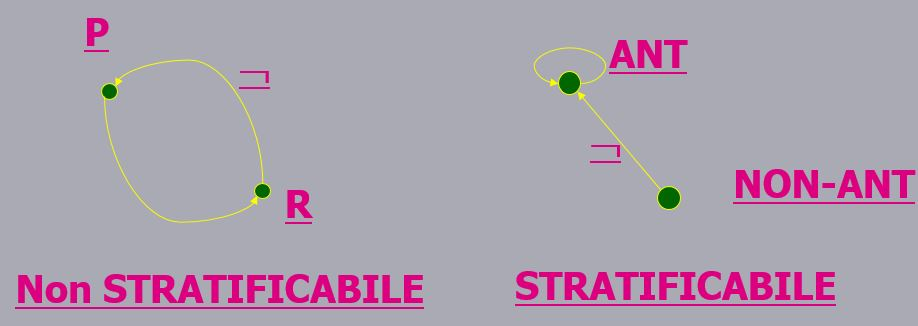
\includegraphics{EsempioProgrammaStratificabile.jpg}
	\caption{Esempi di grafi delle dipendenze di programmi stratificabili e non.}
\end{figure}
\newpage
\subsection{Corrispondenze con il modello relazionale standard}
Possiamo stabilire una corrispondenza tra gli elementi del modello relazionale standard e la terminologia Datalog.\\
\begin{itemize}
\item Relazione $\Rightarrow$ Attributo
\item Attributo $\Rightarrow$ Argomento
\item Tupla $\Rightarrow$ Fatto
\item Query $\Rightarrow$ Regole
\item Interrogazione $\Rightarrow$ Goal
\end{itemize}
\newpage
\section{Structured Query Language (SQL)}
Il nome SQL indica un insieme di linguaggi: DDL (Data Definition Language) e DML (Data Management Language), utili a definire domini, tabelle, indici, autorizzazioni, viste, vincoli, procedure, trigger (DDL) e a scrivere Query, modificare la struttura di un database già formato, scrivere comandi transazionali.
\subsection{Definizione degli Schemi}
Per Schema si intende una collezione di oggetti: domini, tabelle, indici, asserzioni, viste, privilegi, con \bf nome e proprietario\rm.\\ Un esempio di Schema è $$ \tt create\ schema \rm\ [\ \it Nome Schema \rm\ ] $$ $$[\ [\ \tt authorization\rm\ ]\ Autorizzazione\ ]$$ $$\{\ DefinizioneElementoSchema\ \}$$
\subsection{Query SQL}
\subsubsection{Interrogazioni Nidificate}
In termini semplici. è un blocco SQL "dentro" un blocco SQL. Il meccanismom è simile a quello della ricorsione. Esistono 3 modi per nidificare le Query SQL:\\
\paragraph{Nella clausola Where} con i predicati ANY, ALL, o altri operatori di comparazione.\\
L'operatore ANY rende vera l'espressione se esiste almeno una tupla che soddisfa la condizione.\\
L'operatore ALL rende vera l'espressione se tutte le tuple soddisfano la condizione.\\
Esempio di query con ANY ed ALL misti ad altri operatori:
$$ \tt select\ CodOrd $$ $$ \tt from\ Ordine $$ $$ \tt where\ Importo\ \bf >\ any \tt $$ $$ Query\ annidata $$ $$ \tt select\ Importo $$ $$ \tt from\ Ordine $$ \newpage
$$ \tt select\ CodOrd $$ $$ \tt from\ Ordine $$ $$ \tt where\ Importo\ \bf \ge ALL \tt $$ $$ Query\ annidata $$ $$ \tt select\ Importo $$ $$ \tt from\ Ordine $$\\
\paragraph{IN e NOT IN} sono i corrispondendi di = ANY e $\ne$ ALL, sono i concetti intuitivi di appartenenza e non appartenenza ad un insieme.\\
\paragraph{Differenza}
C'è una effettiva differenza tra le quesy nidificate e le loro equivalenti non nidificate a volte. Guarda sulle slide e vedi l'esempio in cui la prima query, quella nidificata, estrae solo una volta il cliente, mentre la seconda che in teoria è equivalente mostra tante volte il cliente quanti sono gli ordini che ha fatto.\\
In teoria ci sono vari modi per scrivere una stessa query, e sono tutti qeuivalenti A MENO DEI DUPLICATI. 
\paragraph{Variabili}
Nelle Query nidificate le variabili possono essere usate per "passare" i valori da una query alla sua sottoquery. Una variabile rappresenta una tupla, posso quindi definire una variabile O in una query e riusarla nella sua sottoquery come O.attributo. Questi strumenti sono molto utili per il push della selezione rispetto al Join\\
Una cosa IMPORTANTISSIMA da tenere a mente quando si decide di usare le variabili in una query con nidificazioni è quella di \bf rispettare le regole di visibilità \rm delle variabili. Come nel C (più o meno), le variabili possono essere utilizzate nella query in cui si definiscono oppure nelle sottoquery ricorsive nidificate direttamente "sotto" di essa, non in altre query ricorsive in un altro livello.
\paragraph{Costruttori di Tupla}
(Nome, Cognome) "costruisce" virtualmente una tupla formata dai parametri Nome e Cognome, che posso poi usare per confrontarla ad esempio con i risultati di una sottoquery che ha la forma $$\tt select\ Nome,\ Cognome$$
\paragraph{Equivalenza del potere espressivo}
Ci sono delle classi di equivalenza tra operatori:\\
IN, =ANY, EXIST\\
NOT IN, $\ne$\ ANY, NOT EXIST\\
"comparatore" ANY, Theta Join (non Equi-Join)\\
"comparatore" ALL, query che abbiano raggruppamento od estrazione di minimo o massimo.
\paragraph{Modifiche}
Le query nidificate ricorsive semplificano molto anche le modifiche dei dati nel database.
\subsubsection{Viste}
Le viste offrono la "visione" di Tabelle Virtuali con schemi diversi da quello del database originale. Sono classificabili in Viste semplici e complesse, quelle semplici hanno solo operazioni di selezione e proiezione su una sola tabella.\\
Possono anche essere usate per realizzare Query, come strumento di modularizzazione, scomponendo una Query in "pezzi" (senza eccedere, ovviemente). Sono anche talvolta \bf necessarie \rm per l'espressione di alcune Query, in particolare quelle che combinano nidificazioni di operatori aggregati diversi. Una volta creata una Vista posso usarla a tutti gli effetti come una Tabella del Database nella scrittura di una Query.\\\\
Le seguanti Quey estraggono il cliente che ha generato il maggior fatturato dal database "Ordini", sono realizzate nel modo "più classico" e la sua forma equivalente con l'utilizzo delle viste.
Query "Classica":
$$\tt select\ CodCli$$
$$\tt from\ Ordine$$
$$\tt group by\ CodCli$$
$$\tt having\ sum(Importo)\ \ge\ ALL\ ($$
$$\tt select\ sum(Importo)$$
$$\tt from\ Ordine$$
$$\tt group by\ CodCli\ )$$
\newpage
Query con View, creazione della Vista:
$$\tt create\ view \ CliFatt(CodCli,\ FattTotale)\ as$$
$$\tt select\ CodCli,\ sum(Importo)$$
$$\tt from\ Ordine$$
$$\tt group by\ CodCli\ )$$
Query con View, scrittura della Query finale:
$$\tt select\ CodCli$$
$$\tt from\ Ordine$$
$$\tt where\ FattTotale\ = \ [ $$
$$\tt select\ max(Fatttotale)$$
$$\tt from\ CliFatt\ ]$$
\\
Ovviamente le viste possono anche essere usate per scrivere Query di modifica del database. La maggiore "differenza" con le Query "normali" è che le operazioni di modifica sulle Viste (una volta create), sono possibili solamente sulle Viste Semplici, mentre non sono possibili su quelle complesse. Un esempio di Query complessa è una qualsiasi Query che usa anche solamente un Join, e il problema fondamentale è che con l'utilizzo del Join (o tutti gli operatori simili) si va a calcolare una tabella con divesre tuple ottenute dalla combinazione delle tuple delle tabelle operando sulla base della condizione. Quindi, volendo aggiornare un parametro che è presnte nella Vista si crea un \bf ambiguità\rm, dato che viene ad essere ambigua la "posizione" del dato da modificare, siccome può essere presente in due tabelle diverse.
\subsubsection{Ricorsione con Viste}
\subsubsection{Controllo dell'Accesso}
L'obiettivo è quello di eseguire un controllo selettivo su chi ha la possibilità di accedere a determinati dati, in modo tale da proteggerli da accessi non autorizzati. Il controllo di accesso e modifica si implementa attraverso il meccanismo delle \bf autorizzazioni\rm.\\\\\\ Copia dalle slide.\\\\ Grant e Revoke. Ciascuno, quando ha la grant option, può passare ad un altro utente solamente i privilegi che ha (ricevuto), non quell che non ha.
\end{document}
